\documentclass[12pt]{article}
\usepackage[utf8]{inputenc}
\usepackage[russian]{babel}
\usepackage{hyperref}
\usepackage{color}
\usepackage{amssymb}
\usepackage{amsmath}
\usepackage{graphicx}

\author{Михаил Лепехин, группа 694}
\title{Домашнее задание №1. Идентификация видов стекла}

\begin{document}
  \maketitle
  
\section*{Постановка задачи}
  $ $
  
Выборка состоит из 9 признаков - химических параметров образцов и 214 объектов. Необходимо каждому образцу сопоставить один из 6 классов (например: стекло автомобиля, осколок посуды, окно здания).

\textbf{Метрика качества}

 Доля правильных ответов классификатора (\textit{accuracy}). 

 Пусть $n$ - количество элементов в тестовой выборке, $y \in \{1, ..., 6\}^n$ - истинные значения классов стекла,  $\widehat{y} \in \{1, ..., 6\}^n$ - предсказания алгоритма.
 
 Тогда \textit{accuracy} можно записать следующим образом:
 
 $$accuracy = \frac{1}{n}\sum\limits_{i=1}^n I(y_i=y) $$

\textbf{Цель}

1.$ $ Решить задачу с использованием следующих методов:

1) Алгоритм k ближайших соседей,

2) Алгоритм решающего дерева

и сравнить качество их работы. 

2.$ $ Отмасштабировать признаки и проверить, даст ли такая процедура увеличение значения \textit{accuracy}.

3.$ $ Выбрать наиболее точный из алгоритмов и исследовать зависимость \textit{accuracy}, достигаемое этим алгоритмом на разных количествах признаков.  
  
\section*{Метод отбора признаков}  
$ $
Отбор признаков быд производён жадным образом. А именно, будем на каждом шаге из недобавленных признаков выбирать такой, что его добавление максимизирует метрику качества на тесте.
  
\section*{Результаты эксперимента}  
  
$ $  
  
После масштабирования признаков точность метода k ближайших соседей повысилась, а метода решающих деревьев - осталась такой же, как и до масштабирования.

Поскольку точность метода k ближайших соседей оказалась выше, будем в дальнейших экспериментах использовать именно его.  
  
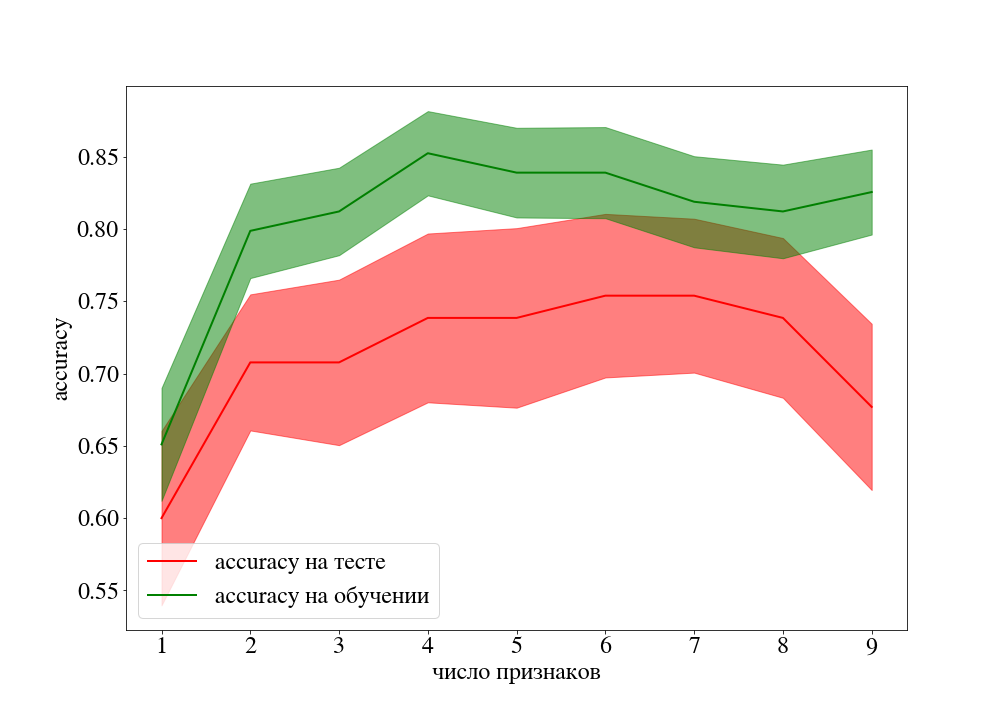
\includegraphics[scale=0.4]{accuracy.png}  
  
\section*{Вывод}

$ $


Как можно увидеть по построенному графику, начиная с 6 признаков, точность работы алгоритма на тестовой выборке начинает ухудшаться. Кроме того, наилучшее значение `accuracy` на обучающей выборке достигается, когда число признаков равно 4.

Это значит, что в данных есть как минимум 3 незначимых признака, от которых необходимо избавиться, чтобы избежать переобучения. 
\end{document}